\documentclass[a4paper,12pt]{report}
\usepackage[T2A]{fontenc}
\usepackage[utf8]{inputenc}
\usepackage[english,russian]{babel}
\usepackage{graphicx}
\usepackage{wrapfig}
\usepackage{mathtext} 				% русские буквы в фомулах
\usepackage{amsmath,amsfonts,amssymb,amsthm,mathtools} % AMS
\usepackage{icomma} % "Умная" запятая: $0,2$ --- число, $0, 2$ --- перечисление
\usepackage{capt-of}
\usepackage{appendix}
\usepackage{multirow}
\usepackage{hyperref}
\usepackage[left=2cm,right=2cm,
    top=2cm,bottom=2cm,bindingoffset=0cm]{geometry}
\usepackage{multicol} % Несколько колонок
\usepackage{gensymb}
\title{Отчёт по лабораторной работе №4.1.1 

Изучение центрированных оптических систем.}
\author{Плюскова Н.А. Б04-004 }
\date{\today}

\begin{document}

\maketitle

\section*{\huge{Описание работы}}
\noindent\textbf{Цель работы:} изучить методы определения фокусных расстояний
линз и сложных оптических систем; определить характеристики оптической системы, составленной из тонких линз; изучить недостатки
реальных линз — сферическую и хроматическую аберрации.

\noindent\textbf{В работе используются:} оптическая скамья с набором рейтеров, положительные и отрицательные линзы, экран, осветитель с ирисовой
диафрагмой, зрительная труба, светофильтры, кольцевые диафрагмы, линейка.

\subsection*{Экспериментальная установка:} 

Оптическая скамья с осветителем,
транспарант, набор линз, экран и зрительная труба позволяют определить параметры оптических систем всеми описанными способами. Все
оптические элементы устанавливаются на скамье при помощи рейтеров.
Важную роль играет правильная центрировка элементов системы.
Проходя через плохо отцентрированную систему, лучи света могут отклониться и пройти мимо экрана или глаза наблюдателя. Центрировать
линзы следует как по высоте, так и в поперечном направлении, для чего
линзы установлены на поперечных салазках.

\subsection*{Аннотация и теоретическое введение:}

\noindent\textbf{I. Определение фокусного расстояния тонкой собирающей линзы
и сложных оптических систем по методу Аббе}

Измерение фокусного расстояния по методу Аббе основано на определении поперечного увеличения для нескольких (не менее двух) различных положений предмета, находящегося на оптической оси исследуемой оптической системы. На рис. 1 представлена соответствующая схема эксперимента.
\begin{center}
    \includegraphics[scale = 1.2]{pic1.PNG}
    \captionof{figure}{Измерение фокусного расстояния оптической
системы по методу Аббе}
\end{center}

Фокусное расстояние системы можно выразить через положения предмета и соответствующие увеличения следующим образом:
\begin{equation}
    f = \frac{\Delta x}{\Delta(y/y')} = - \frac{\Delta x'}{\Delta(y'/y)}. 
\end{equation}

Для повышения точности измерений следует выбирать такие смещения $\Delta x$, чтобы увеличения заметно
отличались друг от друга. С целью уменьшения случайной ошибки,
возникающей при фокусировке изображения, измерения следует проводить несколько раз, усредняя полученные данные.

\newpage
\noindent\textbf{II. Определение фокусного расстояния собирающих линз и сложных
оптических систем по методу Бесселя}
Схема метода Бесселя для случая, когда $n = n'$ и $f' = -f$, представлена на рис. 2. Она основана на том, что при заданном расстоянии $L$ между предметом и экраном уравнение $-1/s + 1/s' = 1/f$  представляет собой квадратное уравнение относительно расстояния s от главной плоскости пространства предметов до предмета (s < 0):
\begin{equation*}
    -\frac{1}{s} + \frac{1}{L-\delta+s} = \frac{1}{f}
\end{equation*}


\begin{center}
    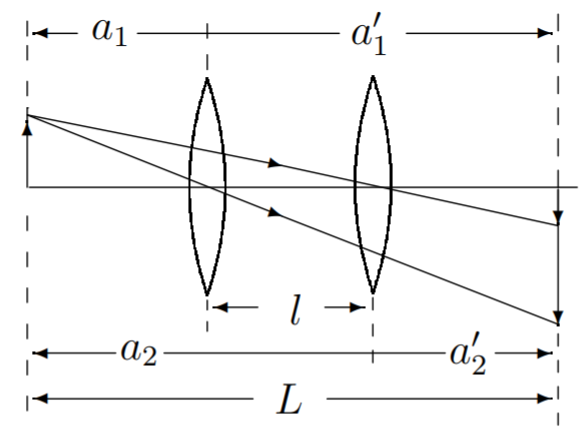
\includegraphics[scale = 0.5]{pic2.PNG}
    \captionof{figure}{Измерение фокусного расстояния оптической
системы по методу Бесселя}
\end{center}

После несложных преобразований находим выражение: 
\begin{equation}
    f = \frac{(L - \delta)^{2} - l^{2}}{4(L - \delta)}
\end{equation}
Если выполняется условие $|\delta| \ll L$, то формула (2) может быть представлена в более простом виде:
\begin{equation}
    f = \frac{L^{2} - l^{2}}{4L}
\end{equation}

Для определения фокусного расстояния $f$ достаточно, таким образом, измерить расстояние $L$ между предметом и экраном и расстояние $l$
между двумя положениями системы, при которых на экране видны чёткие изображения. Допускаемая при этом относительная погрешность
результата измерений (без учёта случайных ошибок) даже для толстых
линз и некоторых сложных оптических систем может быть мала.

\vspace{\baselineskip}
\noindent\textbf{III.  Определение фокусного расстояния тонкой собирающей линзы}
\vspace{\baselineskip}

\noindent\textbf{Способ 1.} 

Воспользуемся формулой тонкой линзы:
\begin{equation}
    -\frac{1}{a} + \frac{1}{a'} = \frac{1}{f}.
\end{equation}
Для измерения фокусного расстояния достаточно провести измерения по стандартной схеме «предмет — линза — экран» при произвольном расстоянии между предметом и экраном с различными значениями $a$ при увеличенном и при уменьшенном изображении. Относительная погрешность определения фокусного расстояния линзы по этому методу порядка $d/f$, где $d$ — толщина линзы. Сравнение среднеквадратичного отклонения измеренных значений $f$ от среднего $d$ позволит сделать
вывод о том, нужны ли многократные измерения

\noindent\textbf{Способ 2.} Фокусное расстояние тонкой собирающей линзы можно
определить с помощью зрительной трубы, настроенной на бесконечность, то есть на параллельный пучок лучей. Разместив между предметом и зрительной трубой положительную линзу и перемещая её вдоль
оси системы, можно найти резкое изображение предмета в окуляре зрительной трубы. При этом расстояние от середины линзы до предмета
равно фокусному расстоянию тонкой линзы. Для толстой линзы зрительная труба позволяет определить только положение главного фокуса.

\vspace{\baselineskip}
\noindent\textbf{IV.   Определение фокусного расстояния тонкой рассеивающей линзы}
\vspace{\baselineskip}

\noindent\textbf{Способ 1.} Определение фокусного расстояния рассеивающей линзы затруднено тем, что изображение предмета получается мнимым
(при действительном источнике) и поэтому не может быть получено
на экране. Эту трудность легко обойти с помощью вспомогательной
собирающей линзы.

\begin{center}
    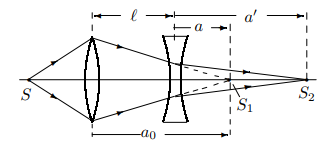
\includegraphics[scale = 1]{pic3.PNG}
    \captionof{figure}{Измерение фокусного расстояния
рассеивающей линзы}
\end{center}
Определив расстояния $a = a_{0} - l > 0$ и $a' > 0$, рассчитывают фокусное расстояние рассеивающей линзы по формуле (3), которое, естественно, должно получиться отрицательным.

\vspace{\baselineskip}
\noindent\textbf{Способ 2.} Если расстояние a на рис. 3 совпадает с модулем фокусного
расстояния рассеивающей линзы, то изображение $S_{2}$ перемещается в
бесконечность, то есть лучи выходят из линзы параллельным пучком.
Параллельность пучка можно установить с помощью зрительной
трубы, настроенной на бесконечность. Зная расстояние от первой линзы
до точки $S_{1}$ и расстояние между линзами, нетрудно определить фокусное расстояние тонкой рассеивающей линзы. Для толстой отрицательной линзы этот метод позволяет определить только положение главного
фокуса.

\vspace{\baselineskip}
\noindent\textbf{V. Определение положения главных и фокальных плоскостей сложной
оптической системы}

Для нахождения главных плоскостей системы недостаточно знать
фокусное расстояние, нужно определить ещё положения главных фокусов. Это можно сделать при помощи зрительной трубы, настроенной на
бесконечность. Отложив от главных фокусов отрезки, равные фокусному расстоянию, можно найти положения главных плоскостей системы.
При этом необходимо учитывать возможность различного взаимного
расположения кардинальных точек (плоскостей) сложной системы.

Все характеристики оптической системы, состоящей из двух тонких
линз, можно рассчитать, если известны фокусные
расстояния $f_{1}, f_{2}$ каждой линзы и оптический интервал $\Delta$ или расстояние между центрами линз $l_{12}$.

\newpage
\vspace{\baselineskip}
\noindent\textbf{VI. Основные аберрации оптических систем}\\

\noindent\textbf{1. Сферическая аберрация}

Сферическая аберрация возникает при преломлении широких (непараксиальных) пучков света на сферических поверхностях линз.Лучи 1, 2, 3, преломляющиеся в линзе на различных расстояниях от центра, пересекают оптическую ось в точках $S_{1}$, $S_{2}$, $S_{3}$. Поэтому преломленные пучки лучей не гомоцентричны; на экране Э вместо точечного изображения получается расплывчатое пятно - кружок рассеяния.
\begin{center}
    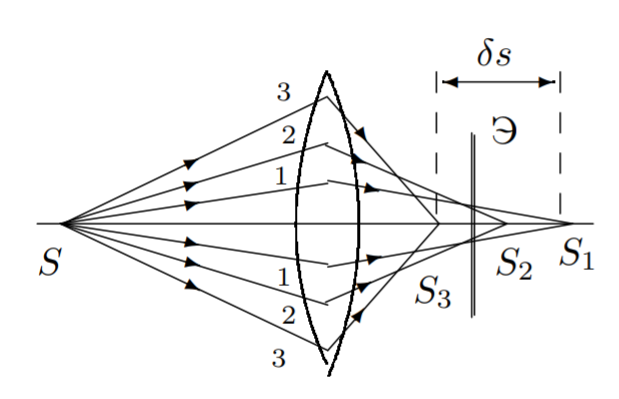
\includegraphics[scale = 0.5]{pic5.PNG}
    \captionof{figure}{Сферическая аберрация}
\end{center}

\noindent\textbf{2. Хроматическая аберрация}

Хроматическая аберрация - зависимость фокусного расстояния линзы от длины волны - возникает вследствие дисперсии показателя преломления стекол, то есть из-за того, что показатель преломления зависит от длины волны света $n = n(\lambda)$. В результате хроматической аберрации на экране Э возникает окрашенный кружок.
\begin{center}
    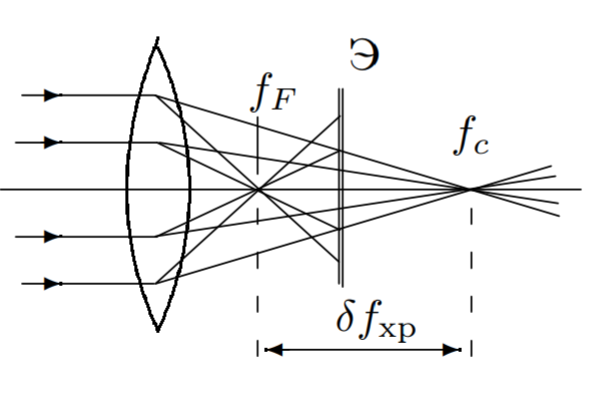
\includegraphics[scale = 0.5]{pic6.PNG}
    \captionof{figure}{Хроматическая аберрация}
\end{center}
Для характеристики дисперсионных свойств стекол часто пользуются \textit{коэффициентом дисперсии}, или \textit{числом Аббе}:
\begin{equation}
    \nu = \frac{n_{D}-1}{n_{F}-n_{C}},
\end{equation}
где $n_{F}$, $n_{C}$ - показатели преломления для голубой, красной линий водорода, $n_{D}$ - показатель преломления для желтой линии натрия.

Хроматическую аберрацию принято характеризовать разностью фокусных расстояний для двух характерных спектральных линий водорода, расположенных в крайних частях видимой области спектра (голубая F и красная C линии).
\begin{equation}
    \delta f_{xp} = f_{F}-f_{C}.
\end{equation}

\newpage
\section*{\huge{Выполнение работы}}

\noindent\textbf{I. Центрировка элементов оптической системы}

Оценим примерное фокусное расстояние собирающих линз. Оценка для первой линзы - $f_{1} \approx 10 $ см; для второй - $f_{2} \approx 15$ см. Фокусное расстояние для третьей линзы было дано изначально - $f_{3} = 8$ см. Стоит заметить, что третья линза использовалась только в опыте с аберрацией, которые мы провели качественном, поэтому фокусное расстояние третьей линзы нам в итоге нигде не понадобилось.

\vspace{\baselineskip}
\noindent\textbf{II. Определение фокусных расстояний тонких линз при помощи экрана}

Определим фокусное расстояние собирающей линзы методом Бесселя. Опыт был проведен для собирающей линзы $\text{Л}_{1}$. Для этого мы расположили экран на расстоянии $L >4f_{1}$ от предмета. Перемещая линзу вдоль скамьи, получили увеличенное и уменьшенное изображения предмета на экране. Полученные значения для опыта с собирающей линзой сведем в таблицу:

\begin{table}[h!]
\centering
\begin{tabular}{|l|l|l|l|l|l|l|}
\hline
Величина & $L, \text{см}$             & $<a_{1}>, \text{см}$            & $<a_{1}'>, \text{см}$           & $<a_{2}>, \text{см}$            & $<a_{2}'>, \text{см}$           & $l, \text{см}$             \\ \hline
Значение & $55.0\pm 0,1$ & $14,1\pm0,1 $ & $40,6\pm0,1 $ & $41,1\pm0,1 $ & $13,7\pm0,1 $ & $27,1\pm0,1 $ \\ \hline
\end{tabular}
\end{table}

Рассчитаем фокусное расстояние линзы №1 по формуле (3) и (4):
\begin{equation*}
    f_{(3)} = \frac{L^{2} - l^{2}}{4L} = \frac{55^{2} - 27,1^{2}}{4\cdot 27,1} = 10,41 \text{ см} \approx (10,4 \pm 0,2) \text{ см}
\end{equation*}

\begin{equation*}
    f_{(4)} = \frac{a\cdot a'}{a + a'} = \frac{14,1 \cdot 40,6}{14,1 + 40,6} = 10,45 \text{ см} \approx (10,5 \pm 0,2) \text{ см}
\end{equation*}

Как можем заметить, значения, найденные двумя разными способами, совпадают в пределах погрешностей.

Теперь рассчитаем фокусное расстояние рассеивающей линзы. Найденные расстояния приведены в таблице ниже: 
\begin{table}[h!]
\centering
\begin{tabular}{|l|l|l|l|l|}
\hline
Величина & $a_{0},  \text{см}$           & $a',  \text{см}$           & $l,  \text{см}$            & $a=a_{0}-l,  \text{см}$      \\ \hline
Значение & $33,1\pm0,1$ & $20,4\pm0,1$ & $24,7\pm0,1$ & $8,4\pm0,1$ \\ \hline
\end{tabular}
\end{table}

Аналогично, рассчитаем фокусное расстояние рассеивающей линзы по формуле (4):

\begin{equation*}
    f = \frac{a\cdot a'}{a + a'} = \frac{-8,4 \cdot 20,4}{-8,4 + 20,4} \approx (14,3 \pm 0,3)\text{ см}
\end{equation*}

\vspace{\baselineskip}
\noindent\textbf{III. Определение фокусных расстояний тонких линз с помощью
зрительной трубы}

Для того, чтобы определить фокусные расстояния линз с помощью зрительной трубы, необходимо было настроить трубу на бесконечность. Настроив трубу и отцентрировав систему, поставим линзу на расстоянии, близком к фокусному, от предмета. Передвигая линзу вдоль скамьи, мы нашли чёткое изображение предмета. Затем мы повернули линзу другой стороной и проделали те же действия. В таблицу ниже занесены найденные значения для двух собирающих линз: 

\begin{table}[h!]
\centering
\begin{tabular}{|l|l|l|l|l|c|c|}
\hline
Величина & $f_{1},  \text{см}$ & $f_{1}^{r},  \text{см}$ & $f_{2},  \text{см}$ & $f_{2}^{r},  \text{см}$ & $<d_{1}>, \text{ дптр}$ & $<d_{2}>, \text{ дптр}$\\ \hline
Значение & $10,8\pm0,1$ & $10,5\pm0,1$  & $12,8\pm0,1$ & $13,1\pm0,1$ & $9,4$ & $13$ \\ \hline
\end{tabular}
\end{table}

\newpage
Для определения фокусного расстояния тонкой рассеивающей линзы была использована собирающая линза. Собрав всю систему, мы измерили следующие расстояния:

\begin{table}[h!]
\centering
\begin{tabular}{|l|l|l|l|l|l|c|}
\hline
Величина & $a_{0}, \text{ см}$           & $l, \text{ см}$           & $l^{r}, \text{ см}$           & $f_{-}, \text{ см}$            & $f_{-}^{r}, \text{ см}$ & $<d>, \text{ дптр}$          \\ \hline
Значение & $34,1\pm0,1$ & $21,6\pm0,1$ & $21,5\pm0,1$ & $-12,5\pm0,1$ & $-12,6\pm0,1$ & -8 \\ \hline
\end{tabular}
\end{table}

\noindent\textbf{IV. Определение фокусного расстояния и положения главных и
фокальных плоскостей сложной оптической системы}

Здесь сложной оптической системой выступают две собирающие линзы, сдвинутые на максимально возможное расстояние. Расстояние между линзами - $l_{12} = 5,2 \text{см}$

Найдем фокусное расстояние этой системы методом Аббе, по найденным перемещениям и изменениям изображения предмета. Ниже представлены значения измерений и расчеты фокусного расстояния по формуле (1):

\begin{table}[h!]
\centering
\begin{tabular}{|l|l|l|c|l|}
\hline
$\text{№ положения}$ & $x, \text{см}$   & $x', \text{см}$   & \multicolumn{1}{l|}{$y, \text{см}$} & $y', \text{см}$   \\ \hline
1         & $7,8\pm0,1$ & $21,6\pm0,1$ & \multirow{2}{*}{2}     & $5,3\pm0,1$  \\ \cline{1-3} \cline{5-5} 
2         & $6,0\pm0,1$   & $48,3\pm0,1$ &                        & $15,6\pm0,1$ \\ \hline
\end{tabular}
\end{table}

\begin{equation*}
    f = \frac{\Delta x}{\Delta(y/y')} = \frac{6,0 - 7,8}{\frac{2}{15,6} - \frac{2}{5,3}} = \frac{-1,8}{-0,25} = (7,2 \pm 0.3) \text{ см} \approx 7 \text{ см} 
\end{equation*}
\begin{equation*}
    f' = -\frac{\Delta x'}{\Delta(y'/y)} = - \frac{48,3 - 21,6}{\frac{15,6}{2} - \frac{5,3}{2}} = -\frac{26,7}{-4} = (6,7 \pm 0.01) \text{ см} \approx 7 \text{ см}
\end{equation*}

Чтобы найти главные фокусы системы, мы закрепили зрительную трубу за второй линзой и, медленно отодвигая источник, нашли четкое изображение предмета. 

Положение главного фокуса системы в пространстве предметов относительно первой линзы $F_{1\Sigma} = 4,9 \text{см}$

Положение главного фокуса системы в пространстве изображений $F_{2\Sigma} = 3,9 \text{см}$

Чёртеж системы изображен на рис.6.

\noindent\textbf{V. Основные аберрации оптических систем}

В идеальных оптических системах лучи, вышедшие из одной точки
объекта, пересекаются в одной и той же точке изображения независимо от угла испускания и длины волны света. В реальных системах такие зависимости имеют место, из-за чего заметно ухудшается качество
изображения. Основные погрешности при этом возникают из-за сферической и хроматической аберраций линз, входящих в состав оптических
систем.

В этом пункте работы мы качественно проделали опыт с аберрацией. Мы увидели как происходит размытие изображения с помощью диафрагм различных диаметров и трех светофильтров (красного, желтого и синего), а также на опыте убедились, что фокусы для разных длин волн и диафрагм различного радиуса немного, но различаются.

\section*{Вывод}

В этой работе мы изучили различные методы определения фокусных расстояний тонких линз и сложных оптических систем. Результаты эксперимента показали, что наиболее точным методом определения фокусного расстояния является метод Бесселя, т.к. значения, полученные методом Аббе имели большее расхождение. Также мы качественно убедились в наличии аберрации в реальных системах.

\begin{center}
    \includegraphics[width = \linewidth]{pic4.jpg}
    \captionof{figure}{Чертёж оптической системы}
\end{center}
\end{document}
